\documentclass[conference]{IEEEtran}

%\usepackage{natbib}
\usepackage{multirow}
\usepackage{mathtools}
\usepackage{fixltx2e}
\usepackage{amssymb}
\usepackage{graphics}
\usepackage{balance}

\title{Real-Time Scheduling algorithms and battery consumption for mobile devices}

\author{\IEEEauthorblockN{David S\'anchez Alb\'an,   Natalia Mar\'in P\'erez,   Luis Diego Chavarr\'ia Ledezma,   Bryant \'Alvarez Canales}
\IEEEauthorblockA{Ingenier\'ia en Computaci\'on\\
Instituto Tecnol\'ogico de Costa Rica\\
San Jos\'e, Costa Rica}
}

\begin{document} 
% make the title area
\maketitle


\begin{abstract}
%\boldmath
With the explosive growth of the mobile devices in the last years, the life of the battery is more important than ever. It has become so important in mobile devices that it is now a challenge for the manufacturers since it is a prominent feature on the market. Besides the improvements on hardware, it has evolved at the software level to even be included as another of the main assets that the OS has to manage along with the CPU, memory, IO and information storage. There has been research on Real-Time Dynamic Voltage Scaling for embedded operating systems that takes care of applying algorithms capable of modifying the OS's real-time scheduler and task management service, this helps to save energy greatly. Real Time Scheduling algorithms have improved the efficiency of the embedded systems and also tuning the CPU configuration has helped to consume less power without missing any deadline. In this paper we explore different algorithms for real time scheduling and how they can impact, in a good or a bad way, the energy consumption and the battery’s life and we  propose a novel way to improve these scheduling algorithms using the profile information recollected by the OS about energy consumption and the relevance of the app to the user, allowing us to find the deadlines that need to be met in order to improve the energy savings.
\end{abstract}

\section{Introduction}

The battery lifetime is an important factor in assessing the users satisfaction on a mobile consumer electronic product. In recent years, the real-time systems have been integrated to a wide range of applications. Due to its complexity this type of systems they provide high reliability, with the right results and they are predictable and since they need to meet a deadline, it is always on time, helping to minimize the battery consumption.\cite{MANISH} \\
In the mobile devices, the greatest obstacle is the battery lifetime, which restricts the system function to a limit period of time. 
Our investigation has the intent of taking advantage of the new technologies and scheduling algorithms to manage the energy in mobile systems where the multiprocessor is capable of operate in different voltage levels which would implicate different level of energy consumption.\cite{PADM01}\\
To demonstrate that these systems operate with this restrictions, we will prove that every task of critical time that are part of the system will deliver results in the appropriate time, with the expected outcome, in a predictable way and without failures. 
In order to resolve this problem we will develop a new algorithm, with new design tools and real-time software validation systems.

The specific objectives of this investigation are:
\begin{itemize}
\item Propose a novel solution to the scheduling of dynamic tasks in mobile devices and minimize the energy consumption of the total amount of tasks on the system.
\item Monitor the battery capacity dynamically, the energy consumption on different components of the system and the frequency of when the battery gets recharged.
\item Develop new models and algorithms in real-time systems with the energy consumption and fault tolerance restrictions.
\end{itemize}


This paper focuses on saving energy by modifying the OS real-time scheduler and how it can be implemented securely and efficiently. 
Section 2 provides a more detailed background about the challenges with real time scheduling and their impact on the devices' battery life. Section 3 discusses about the mobile devices and power management. Section 4 explains the scheduling algorithm to manage better the battery consumption on mobile devices. Sections 5 summarizes related work and Section 6 concludes.

\section{Background}
\subsection{Background of real-time systems}
The greatest objective of real-time systems is to meet on time their activities to satisfy the requirements of their application. So the design of those systems should be capable of analyse the characteristics of the real-time tasks and extract their requirements to have the system ensure schedulability, which means, meeting the deadlines in all the tasks in its execution. \cite{STAN01} \\
A real-time application is composed by a number of concurrent tasks that cooperate among themselves.  This tasks are activated  on regular and irregular intervals and they have to complete their execution according to a deadline. On each activation, the task completes a computation, and interacts with an external environment. According to the real-time requirements, a task must be: 1) Critical: if not meeting a timed requirement will cause a failure because of its consequences on the system, 2) Uncritical: It is possible to tolerate the failure to meet the deadline of a timed requirement. Some of the attributes of a real-time task are: a) maximum time of computation which is given by the implementation, b) period or frequency of the run and c) the response time, which is defined by the application attributes. Therefore, the tasks can be: periodic, that are executed with a fixed or variable periodicity, and aperiodic, which are run in response to an event that occur on the system at irregular intervals.\cite{AVI01} \\
Naturally these tasks are evaluated based on the algorithm that is being used in order to administer the resources within the system,  for such studies it's important to consider the evaluation methods required, for example, the comparison between RM (Rate-Monotimic) and EDF (Earliest Deadline First) algorithms.\cite{BECKER01} 
The RM algorithm uses a static-priority method, where the shorter the cycle duration is the higher the priority it is, versus the EDF algorithm where the lower the deadline the higher priority it has. 
In order to contrast both algorithms a set of tasks is used in order to evaluate their overhead, for example the algorithm run against 2-4-8 tasks then the CPU frequency, CPU usage, Energy consumption and CPU cycles are compared between one and the other. 
The result provided by  \cite{BECKER01} show that each algorithm has a different purpose, the RM algorithm shows a bigger overhead but a better performance than the EDF which provides a better energy consumption than RM. 
 
 \subsection{Background of mobile devices with energy management}

 With the recent arrival of portable systems and communications, the energy consumption has been a major aspect to consider on the design of these systems. Currently, the market offers functions of energy management that allow to disable certain components or choosing different levels of energy consumption. Besides that, the software and hardware makers have agreed on creating standards like the ACPI (Energy Interface of Advanced Configuration) to handle energy with portable computers, which allow to manage different modes of operation (voltage) on the system. Recent investigation have shown that reduction on memory consumption can be achieved through the dynamic management of frequency/voltage and through compiling techniques and algorithms. \cite{MARGI01} \\
 
 Thanks to the progress in the microprocessors technologies we can see mechanisms on personal computers to disable (shut-down) the computer after detecting long periods of inactivity. In this case the computer changes to an operation mode where the secondary devices are shut-down like disks, screen and some parts of the memory which reduces the energy consumption considerably. This type of multiprocessors are capable to operate on a frequency and voltage range, which allows the system to complete computations to different speeds \cite{PADM01}. The capacity of decrementing the processor velocity allows the system to reduce its memory consumption. The dynamic scheduling of voltage in real-time systems and meeting the timed restrictions has the objective to minimize the energy consumption.

 Minimizing the energy consumption in this kind of system is important because it allows to increase the lifetime of batteries and at the same time it helps to extend the time of the system functionality. On the other hand, given this systems being real-time, the voltage reduction produce an increase in the computation time and this could compromise meeting the deadlines. Because of this, when reducing the energy it is needed to verify that the timed restrictions don't get broken. So, factors that need to be managed on this type of systems are: a) saving the energy, b) voltage levels, c) computation time and d) scheduling of the real-time system.
 
 For example, As shown in the information below \cite{CarrollAnalysis} the smartphones consume energy according specific patterns. 
 "Suspend" represents the baseline case of a device which is on standby, without placing or receiving calls or messages. The casual pattern represents a user who uses the phone for a small number of voice calls and text messages each day. Regular represents a commuter with extended time of listening to music or podcasts, combined with more lengthy or frequent phone calls, messaging and a bit of emailing. The business pattern features extended talking and email use together with some web browsing. Finally, the PMD (portable media device) case represents extensive media playback:

\begin{table}[h]
\resizebox{\columnwidth}{!}{%
\begin{tabular}{|l|c|c|c|c|c|c|}
\hline
Workload & \multicolumn{1}{l|}{SMS} & \multicolumn{1}{l|}{Video} & \multicolumn{1}{l|}{Audio} & \multicolumn{1}{l|}{Phone call} & \multicolumn{1}{l|}{Web browsing} & \multicolumn{1}{l|}{Email} \\ \hline
Suspend  & -                        & -                          & -                          & -                               & -                                 & -                          \\ \hline
Casual   & 15                       & -                          & -                          & 15                              & -                                 & -                          \\ \hline
Regular  & 30                       & -                          & 60                         & 30                              & 15                                & 15                         \\ \hline
Business & 30                       & -                          & -                          & 60                              & 30                                & 30                         \\ \hline
PMD      & -                        & 60                         & 180                        & -                               & \multicolumn{1}{l|}{-}            & \multicolumn{1}{l|}{-}     \\ \hline
\end{tabular}%
}
\caption {Usage patterns, showing total time for each activity in minutes \cite{CarrollAnalysis}.}
\end{table}
  


\begin{table}[h]
\resizebox{\columnwidth}{!}{%
\begin{tabular}{|c|c|c|c|c|c|c|c|c|}
\hline
\multirow{2}{*}{Workload} & \multicolumn{7}{c|}{Power (\% of total)}            & \multirow{2}{*}{\begin{tabular}[c]{@{}c@{}}Battery life\\  {[}hours{]}\end{tabular}} \\ \cline{2-8}
                          & GSM & CPU & RAM & Graphics & LCD & Backlight & Rest &                                                                                      \\ \hline
Suspend                   & 45  & 19  & 4   & 13       & 1   & 0         & 19   & 49                                                                                   \\ \hline
Casual                    & 47  & 16  & 4   & 12       & 2   & 3         & 16   & 40                                                                                   \\ \hline
Regular                   & 44  & 14  & 4   & 14       & 4   & 7         & 13   & 27                                                                                   \\ \hline
Business                  & 51  & 11  & 3   & 11       & 4   & 11        & 10   & 21                                                                                   \\ \hline
PMD                       & 31  & 19  & 5   & 17       & 6   & 6         & 14   & 29                                                                                   \\ \hline
\end{tabular}%
}
\caption{Daily energy use and battery life under a number of usage patterns  \cite{CarrollAnalysis}.}
\end{table}

With this example is possible to observe when managing efficiently the energy through the system components we can achieve a reduction on the voltage consumption.
 
Power management (PM) schemes from the operating system level is a promising method to manage the battery lifetime because the OS is aware of the battery discharging status, the application energy requests as well as the device power states \cite{PADM02}.
 
Other important section is analysis of the GPU algorithms in used in order to save energy, as stated in \cite{ARIUN01}, where they are using different job size in order to reduce the amount of energy being consumed by each algorithm, the larger jobs that are  processed by the GPU assist in processing these at the same time than smaller tasks, due to the fact that the GPU is an throughput-based machine. This phenomenon occurs because the threshold of all computational resources of the GPU are used and does not enhance the performance of the GPU. 
 
\subsection{Scheduling algorithms}
\subsubsection{Dynamic Voltage Scheduling in Real-time systems}
 Dynamic Voltage Scheduling in Real-time systems uses the EDF (Earliest Deadline First) algorithm. For example, on \cite{PADM01} the lookahead RT-DVS EDF algorithm's goal is to defer work beyond the earliest deadline in the system to operate at a low frequency now. The time is allocated in the schedule for the worst-case execution of each task, starting with the task with the latest deadline. The algorithm finds a lower operating frequency. Continuing this method of trying to defer work beyond the next deadline in the system ultimately results in the execution trace.\\
The actual algorithm is as follows:

\noindent\rule{8cm}{0.4pt}
\begin{equation}
$$select\_frequency(x):\\
	use lowest freq  f$_{i}$ $\in$ \{f$_{1}$ ,..., f$_{m}$ | f$_{1}$ $<$ ... $<$ f$_{m}$\}\\
	such that \$x $\leq$ f$_{i}$ / f$_{m}$ $$
$$upon task\_release(T$_{i}$):\\
	set c\_left$_{i}$ = C$_{i}$;\\
	defer();$$
$$during task\_execution(T$_{i}$):\\
	decrement c\_left$_{i}$;$$
$$defer():\\
	set U=C$_{1}$/P$_{1}$ + ... C$_{n}$ + P$_{n}$;\\
	set s=0;\\
	for i=1 to n, T$_{i}$ $\in$ \{T$_{1}$ ,..., T$_{n}$ | P$_{1}$ $\leq$ ... $\leq$ P$_{n}$ \} \\
		if ( c left$_{i}$  $<$ k )\\
			set d$_{i}$  = c\_left$_{i}$;\\
			set k = k - c\_left$_{i}$;\\
		else\\
			set d$_{i}$  = k;\\
			set k = 0;$$
\end{equation}
\noindent\rule{8cm}{0.4pt}

There are other works related to this such as the one proposed by C.M.Krishna and Y.H.Lee \cite{KRISH01} which it is also based on EDF (Earliest Deadline First), there is a processing phase that takes care of looking for a voltage nominal level for the tasks, all tasks' instances start their execution. This phase is based on the tasks that have a maximum computation time. This algorithm has a dynamic phase too, when the tasks need less time time of maximum computation, it looks to assign the execution time that is not assigned to other tasks (which decrements its voltage/energy consumption). 

\subsubsection{Completely Fair Scheduler and Energy-based Fair Queuing scheduling algorithm}

Android uses the same scheduler as Linux, known as Completely Fair Scheduler (CFS) \cite{ANDR01}. CFS provides balance between tasks assigned to a processor. For that, it uses a red-black binary tree,  with self-balancing capabilities.  As the tree is being used for scheduling purposes, the balance factor is the amount of time provided to a given task. This factor has been named virtual runtime. The higher the task’s virtual runtime value, the lower is the need for the processor.\\
In terms of execution, the algorithm works as follows: the tasks with lower virtual runtime are placed on the left side of the tree, and the tasks with the higher virtual runtime are placed on the right. This means that the tasks with the highest need for the processor will always be  stored on the left side of the tree. Then, the scheduler picks the left-most node of the tree to be scheduled. Each task is responsible for accounting the CPU time taken during execution and adding this value to the previous virtual runtime value. Although CFS tries to optimise the time a task is waiting for CPU time, this effort is not enough as it is not capable of providing guaranteed response times. \\
The CFS code is used as base for the The EFQ (Energy-based Fair Queuing) algorithm which assessed from two aspects, energy management and real-time scheduling. 
It is advised that energy should be globally managed as the first-class resource in the system  the corresponding PM (Power Management) schemes are called energy centric PM schemes. An energy-centric PM scheme can ensure a target battery lifetime for user-specified applications by restricting the battery discharging rate over the time and proportionally allocating energy among different applications.  It relies on the cooperation of the energy estimation module, energy accounting module, energy allocation module and energy scheduling module to achieve advanced energy objectives such as lifetime guarantee \cite{WEI01}.

\subsection{Rate-monotonic algorithm}

This algorithm is used in the investigation proposed by \cite{BECKER01}, this algorithm consists of calculating the amount of cycles required to complete a task, which is then evaluated and a static-priority is assigned after that, where the task with the lowest cycle has more priority than the rest. The algorithm is generally preemptive and guarantees response times due to it's behavior while assigning the resources. 
This algorithm is easy to implement a proposes a deterministic model which enables this algorithm to predictable. This algorithm creates a time-table in order to track the processor cycles, however this table creates a big memory overhead, since it can grow exponentially due to the amount of tasks required. Which leads to a bigger use of power due to the extensive amount of memory that is uses, however it excels at running tasks effectively. 


\section{Proposed Scheduling algorithm}

\begin{figure*}[ht]
\centering
  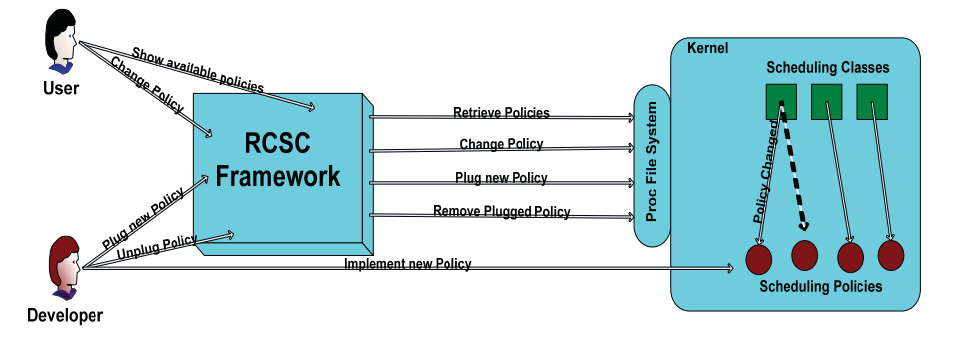
\includegraphics[width=\textwidth,height=4cm]{RSCS}
  \caption{Architecture of RCSC framework \cite{ALMA01}}
  \label{fig:RCSC}
\end{figure*}

In our investigation, first, we want take as a baseline the CPU scheduler framework proposed in \cite{ALMA01}. First we have to extend the RCSC (Real-Time CPU Scheduler Customization) not just to plug policies in runtime, we want it to extend it to enable or disable any policy according to the set of rules that the scheduler will create always keeping the user experience and the battery life as the centre of the algorithm. To create those rules, we will take the data collected from the user, the usage of the devices and some configurations that the user can set, to create a set of policies and then define the rules that will trigger the switching between policies.

As shown on the Figure~\ref{fig:RCSC} the RCSC architecture will  manage the scheduling policies using the CPU scheduler. Important components of the RCSC architecture include:
\begin{itemize} 
\item CPU scheduler
\item Scheduling classes
\item Scheduling policies
\item The proc file system. 
\end{itemize}

Some of the scheduling policies for example are the ones that the existing CFS class encapsulates for example NORMAL, BATCH and IDLE \cite{SchLnx}. 
As such, a new scheduling class can be used to encapsulate new scheduling policy(s). The framework will start scanning for available pluggable scheduling policies  and classes inside a directory of scheduling policies. Each time new scheduling policies and classes are added, the framework must be reinitialized. Scheduling polices is another component of RCSC framework. \\
The policies are the scheduling algorithms which are used to implement the scheduling method i.e. FIFO (First In Firt Out), RR (Round Robin) and SJF (Shortest Job First). They can be dynamically switched from user space, plugged and unplugged to the framework at runtime.  \cite{ALMA01} \\
The proc file system will facilitate the switching between the policies, plugging and unplugging of classes and policies. The framework will maintain a proc file for each policy inside the folder and a proc file for the configuration of the framework itself. When the scheduler is called to decide the CPU control of the next process, the framework will load the specified user scheduling policy to be used by the core scheduler.\\
Since the policies are pluggable during the execution time then the the mobile users or the operating system itself could adapt to the changing requirement.\\

It will record the below metrics from the scheduling algoritm:
\begin{itemize}
\item Arrival time
\item Start time
\item Completion time
\item Computation time
\item Deadlines met
\end{itemize}

The policies will be exchanging among the below scheduling algoritms \cite{GITAM01}
\begin{itemize}
\item FIFO: Processes assigned to the CPU in the order that was requested
\item Shortest Job First: Once the CPU is available, it will allocate the process that has the smallest CPU burst. So, once the process gets to the ready queue the CPU burst will be lower than the current running process 
\item Round-Robin: Each process gets a limited amound of CPU time to execute. If the CPU burst of the process is the same or lower then it will release the CPU. Otherwise, the scheduler will preempt the running process after the limited time and will put it back on the ready queue and dispatch another process from the ready queue.
\end{itemize}

Future work of this topic will cover testing of the RCSC framework and will demonstrate how switching between the scheduling algorithms mentioned above will increase the CPU throughput greatly and energy saving helping to also improve the flexibility and the mobile operating system maintenance. 

\section{Related Work}

There are multiple studies in the energy efficiency category, such as the big.LITTLE mobile processor \cite{KISO01}, which is based of the architecture models for AMP ( Asymmetric MultiProcessing ) and HMP (Heterogeneous MultiProcessing), where this processor is offered as an alternative to the HMP, since two kinds of processors are used in this model, one processor is low power consuming and low throughput, this will be the LITTLE processor, and the big processor is used for high performance/high energy consuming tasks, that require more resources in order to complete the task.
This processor makes use of the CFS (Completely Fair Scheduler) which was introduce in Linux 2.6.23, this is used to run tasks in parallel with with precise weight speeds. 
big.LITTLE makes use of the DVFS (Dynamic Voltage and Frequency Scaling), this is a simple algorithm that is in charge of controlling the voltage and frequency, this changes based on the requirements that the processor needs at an specific time, here is where two specific concepts are introduced overvolting, that is when the processor needs more voltage and frequency and the opposite will be undervolting, when voltage and frequency are lowered. This is mostly used to control the power saving of mobile devices. RCSC (Real-Time CPU Scheduler Customization) \cite{ALMA01} is the key framework that was studied in this paper thanks to its flexibility to manage different policies and scheduling algorithms it helps to manage the CPU more efficiently.

\section{Conclusion}
After this, for real time mobile operating systems we look at various structures, algorithms and standards. We reviewed different algorithms that had been studied to manage battery consumption efficiently  in previous papers but, after reviewing the different algorithms we decided to use the RCSC framework and manage the CPU which is the feature that impacts more the performance and the mobile devices energy consumption according to the according to the analysis discussed previously. \\
In this paper, we propose the use of the RCSC framework along with different scheduling policies. RCSC architecture provides pluggable scheduling policies and important features to customize the mobile operating system to improve the efficiency and energy saving

\nocite{*}


\bibliographystyle{IEEEtranS} %sorted by Author's Name
\bibliography{Real-Time_Scheduling_Algorithms_And_Battery}


\end{document}
